% author:   Ritashugisha
% date:     2015-03-17 17:12:30
% modified: 2015-03-19 19:18:09

\documentclass{article}
\usepackage[margin=0.7in]{geometry}
\usepackage{fancyheadings}
\usepackage{tabularx}
\usepackage{graphicx}
\pagestyle{fancy}
\def\arraystretch{1.5}
\begin{document}
\lhead{Team 3 --- Phase 1}
\begin{center}\textbf{\large Project Description}\end{center}
The objective of this database is to make a user interface that has the ability to create, view, and/or update events such as classes, extra-curricular activies, meetings, etc... that take place in Anne Belk Hall. This database's main use will be to provide convenience and accessibility when checking for room and/or computer availability for scheduling events or personal use. Hopefully, with the assitance of the faculty, we will be able to improve or recreate the building map provided online with additional support and features.\\\\
Our project's database will keep a schedule of the events that occur in each room at what day and time. This database will keep track of event managers along with their scheduled events allowing the managers to add, update, and/or delete their events. Managers will be limited to adding events to rooms that they have permission to access through the use of the permissions field. This permissions field will act as a modified version of unix permissions (ex: 777, 775, etc...).\\\\
We wish to create a versatile framework for this database in order to maybe expand this project to other buildings and events. Hopefully we will be able to complete this project and present a superior product to handle event/room scheduling management.
\\\hline
\begin{center}\textbf{\large Tentative Plan}\end{center}
\begin{description}
    \item[March 20] \hfill Phase 1 due
    \item[March 24]\hfill  Python database framework due
    \item[April 3]\hfill  Django webserver framework due
    \item[April 9]\hfill  Database managing web service due
    \item[April 16] \hfill User interactivity views and templates due
    \item[April 23] \hfill Visual representation of rooms and layout due
    \item[April 30] \hfill Database authentication and visualization due
    \item[May 1]\hfill  Full database project due
\end{description}
\\\hline
\begin{center}\textbf{\large Project Questions}\end{center}
We will be meeting with Paul Wilson (the administrative assistant for the CS Department) to ask questions about specifications and valued features for our project. We will be meeting him at 3:00 PM on 3-25-2015 in Anne Belk Hall room 312P. Here are a few of the questions we came up with before the meeting.
\begin{itemize}
    \item Do you have a pre-existing database we can view and consult?
    \item What sort of specifications do we need to meet to validate this project?
    \item Can we have access to scheduling records for classes and activities?
    \item What features would you appreciate from this database?
    \item Have there been past efforts to create a similar database? If so, what problems occured?
\end{itemize}
\newpage
\begin{center}\textbf{\large Member Responsibilities}\end{center}
\begin{description}
    \item[Stephen Bunn (\emph{Team Leader}, \emph{Development Manager})] \hfill\\ Build and maintain an effective team.\\Motivate all team members to work aggressively on the project.\\Resolve all the issues team members bring to him/her.\\Keep the instructor fully informed about the team's progress.\\Perform effectively as the team's meeting facilitator.\\Produce a superior product.\\Fully use the team members' skils and abilities.
    \item[Chun Zheng (\emph{Support Manager})] \hfill\\ Ensure the team has suitable tools and methods to support its work (software, etc...)\\No unauthorized changes are made to baselined products.\\All team's risks and issues are recorded in the issue-tracking system and are reported each week.
    \item[Austin Mann (\emph{Planning Manager}, \emph{Group Communicator})] \hfill\\ Produce a complete, precise, and accurate plan for the team and every team member.\\Accurately report team status every week.
    \item[Walt Scarboro (\emph{Quality/Process Manager})] \hfill\\ All team members reported possible problems or defects and they are recorded in the project notebook.
\end{description}
\\\hline
\begin{center}\textbf{\large Software and Utilities}\end{center}
\begin{description}
    \item[Python] \hfill High level programming language used as our host language.
    \item[Django] \hfill Python web framework used as our user interface framework.
    \item[Foundation] \hfill HTML bootstrapping framework.
    \item[Sqlite3] \hfill Database framework to create and manage our database.
    \item[SqliteMan] \hfill 3rd party program idrf to debug our database.
\end{description}
\\\hline
\begin{center}\textbf{\large Database Schema}\end{center}
\textbf{\Large BUILDING}\\\\
\begin{tabular}{|c|l|l|l|}
    \hline
    \underline{buildingID} & name & roomcount & floorcount \\ \hline
\end{tabular}\\\\\\
\textbf{\Large ROOM}\\\\
\begin{tabular}{|c|l|l|l|l|l|}
    \hline
    \underline{roomID} & capacity & name & type & permissions & available \\ \hline
\end{tabular}\\\\\\
\textbf{\Large EVENT}\\\\
\begin{tabular}{|c|l|l|l|l|l|l|l|l|l|}
    \hline
    \underline{eventID} & name & timestart & timeend & datestart & dateend & yearly & monthly & weekly & daily \\ \hline
\end{tabular}\\\\\\
\textbf{\Large MANAGER}\\\\
\begin{tabular}{|c|l|l|l|l|l|l|}
    \hline
    \underline{managerID} & namefirst & namemiddle & namelast & email & permissions & sex \\ \hline
\end{tabular}\\\\\\
\textbf{\Large PERIPHERAL}\\\\
\begin{tabular}{|c|l|l|l|}
    \hline
    \underline{peripheralID} & name & working & permissions \\ \hline
\end{tabular}\\\\\\
\newpage
\begin{center}\textbf{\large Database Catalog}\end{center}
\textbf{\Large BUILDING}\\\\
\begin{tabularx}{\textwidth}{|X|X|X|X|}
    \hline
    \textbf{\large Name} & \textbf{\large Data Type} & \textbf{\large NOT NULL} & \textbf{\large Primary/Foreign} \\ \hline buildingID & INTEGER & NOT NULL & Primary \\ \hline name & TEXT & NOT NULL & \\ \hline roomcount & INTEGER & NOT NULL & \\ \hline floorcount & INTEGER & NOT NULL & \\ \hline
\end{tabularx}\\\\\\
\textbf{\Large ROOM}\\\\
\begin{tabularx}{\textwidth}{|X|X|X|X|}
    \hline
    \textbf{\large Name} & \textbf{\large Data Type} & \textbf{\large NOT NULL} & \textbf{\large Primary/Foreign} \\ \hline roomID & INTEGER & NOT NULL & Primary \\ \hline capacity & INTEGER & & \\ \hline name & TEXT & NOT NULL & \\ \hline type & TEXT & & \\ \hline permissions & INTEGER & NOT NULL & \\ \hline buildingID & INTEGER & NOT NULL & Foreign \\ \hline
\end{tabularx}\\\\\\
\textbf{\Large EVENT}\\\\
\begin{tabularx}{\textwidth}{|X|X|X|X|}
    \hline
    \textbf{\large Name} & \textbf{\large Data Type} & \textbf{\large NOT NULL} & \textbf{\large Primary/Foreign} \\ \hline eventID & INTEGER & NOT NULL & Primary \\ \hline name & TEXT & NOT NULL & \\ \hline timestart & REAL & NOT NULL & \\ \hline timeend & REAL & NOT NULL & \\ \hline datestart & REAL & NOT NULL & \\ \hline dateend & REAL & NOT NULL & \\ \hline yearly & INTEGER & NOT NULL & \\ \hline monthly & INTEGER & NOT NULL & \\ \hline weekly & INTEGER & NOT NULL & \\ \hline daily & INTEGER & NOT NULL & \\ \hline managerID & INTEGER & NOT NULL & Foreign \\ \hline roomID & INTEGER & NOT NULL & Foreign \\ \hline buildingID & INTEGER & NOT NULL & Foreign \\ \hline
\end{tabularx}\\\\\\\\\\\\\\\\\\
\textbf{\Large MANAGER}\\\\
\begin{tabularx}{\textwidth}{|X|X|X|X|}
    \hline
    \textbf{\large Name} & \textbf{\large Data Type} & \textbf{\large NOT NULL} & \textbf{\large Primary/Foreign} \\ \hline managerID & INTEGER & NOT NULL & Primary \\ \hline namefirst & TEXT & NOT NULL & \\ \hline initialmiddle & TEXT & & \\ \hline namelast & TEXT & NOT NULL & \\ \hline email & TEXT & NOT NULL & \\ \hline sex & TEXT & & \\ \hline permissions & INTEGER & NOT NULL & \\ \hline 
\end{tabularx}\\\\\\
\textbf{\Large COMPUTER}\\\\
\begin{tabularx}{\textwidth}{|X|X|X|X|}
    \hline
    \textbf{\large Name} & \textbf{\large Data Type} & \textbf{\large NOT NULL} & \textbf{\large Primary/Foreign} \\ \hline computerID & INTEGER & NOT NULL & Primary \\ \hline name & TEXT & NOT NULL & \\ \hline working & INTEGER & NOT NULL & \\ \hline permissions & INTEGER & NOT NULL & \\ \hline  roomID & INTEGER & NOT NULL & Foreign \\ \hline
\end{tabularx}\\\\\\
\begin{center}\textbf{\large Database ER Diagram}\end{center}
\begin{figure}[ht!]
\centering
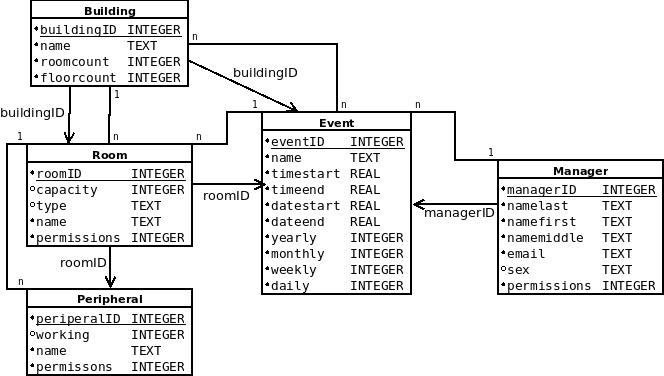
\includegraphics[width=150mm]{erumldia.jpg}
\end{figure}

\end{document}